\chapter{Risk Management}
\section{Risk Management Plan}
\justifying
\parindent20pt The CHSRA adheres to a formal risk management process that aligns with the ISO 31000 standards. The process involves: \begin{itemize}
	\item \textbf{Risk Identification}: Conducted through expert workshops, historical data analysis, stakeholder interviews, and scenario simulations.
	\item \textbf{Risk Assessment}: Risks are evaluated in terms of likelihood and impact using a qualitative and quantitative matrix.
	\item \textbf{Risk Response Planning}: Strategies are developed, including mitigation, transfer, acceptance, or avoidance.
	\item \textbf{Risk Monitoring and Control}: Continuous monitoring through regular reviews, updates, and use of Early Warning Systems (EWS).
\end{itemize}

\newpage
\section{Risk Management and Mitigation Matrix}

\noindent %\vspace*{0.2em}
\begin{center}
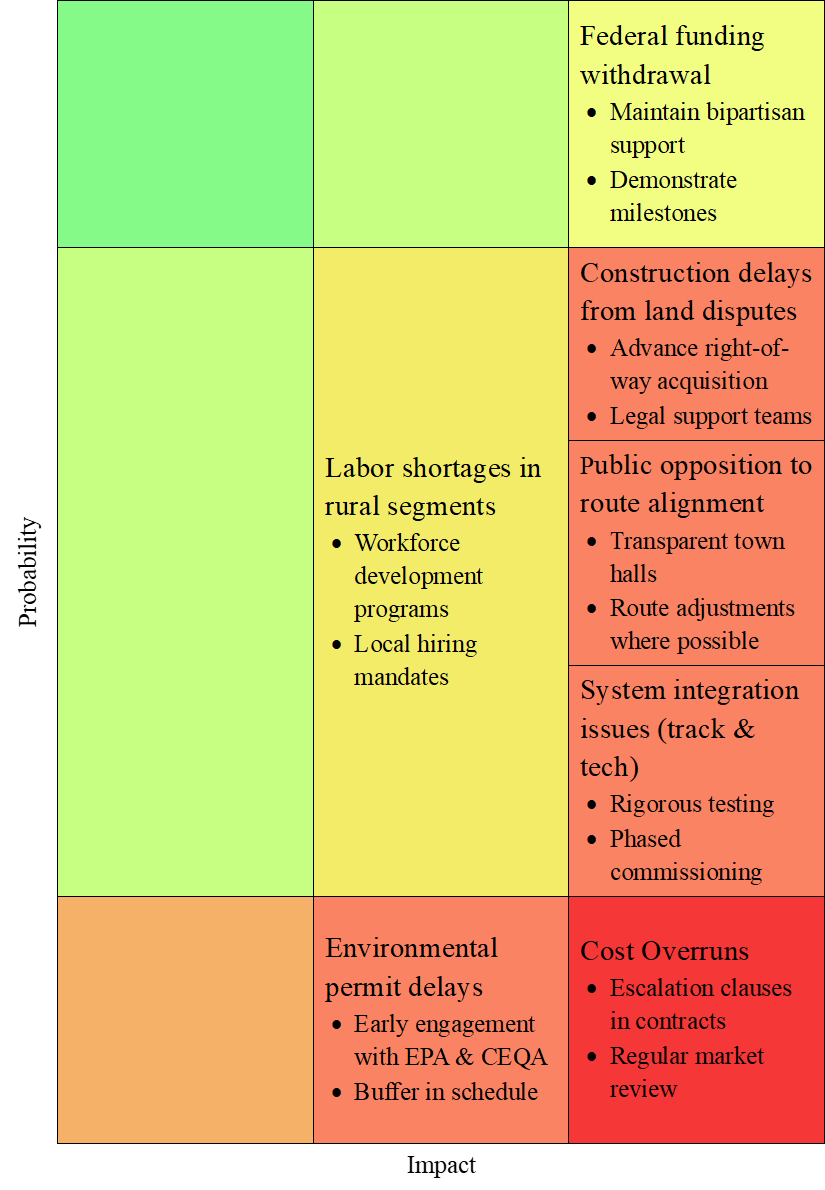
\includegraphics[width=0.8\linewidth]{./attachments/probimp} \vspace*{0.5em}
\end{center}\par
\justifying